\documentclass[12pt,letterpaper]{hmcpset}
\usepackage[margin=1in]{geometry} 
\usepackage{graphicx}
\usepackage{amsmath}
\usepackage{boxedminipage}
\usepackage{url}
\usepackage{geometry}

% info for header block in upper right hand corner
\name{}
\class{Math 45 - Section --- \hspace{20pt}}
\assignment{HW 08}
\duedate{Friday, April 15, 2016}

\newcommand{\pn}[1]{\left( #1 \right)}
\newcommand{\abs}[1]{\left| #1 \right|}
\newcommand{\bk}[1]{\left[ #1 \right]}

% Start enumerates at a) instead of 1
\renewcommand{\labelenumi}{{(\alph{enumi})}}

%Block Paragraphs
\setlength{\parindent}{0pt}
\setlength{\parskip}{1em}

\begin{document}

\problemlist{1, 2, 3, 4, 5}

\begin{problem}[1]
    Examine Student Z's work on the following problem.  What did the student do correctly?  What mistake(s) did the student make?  What is a more correct response to the problem, and what would you say to help the student understand how to correctly complete the problem?

    \begin{center}
        \framebox{\parbox[c]{5.5in}{Determine the solution to the IVP $y'=-x+y$ with $y(\sqrt{2})=0$.

        \centering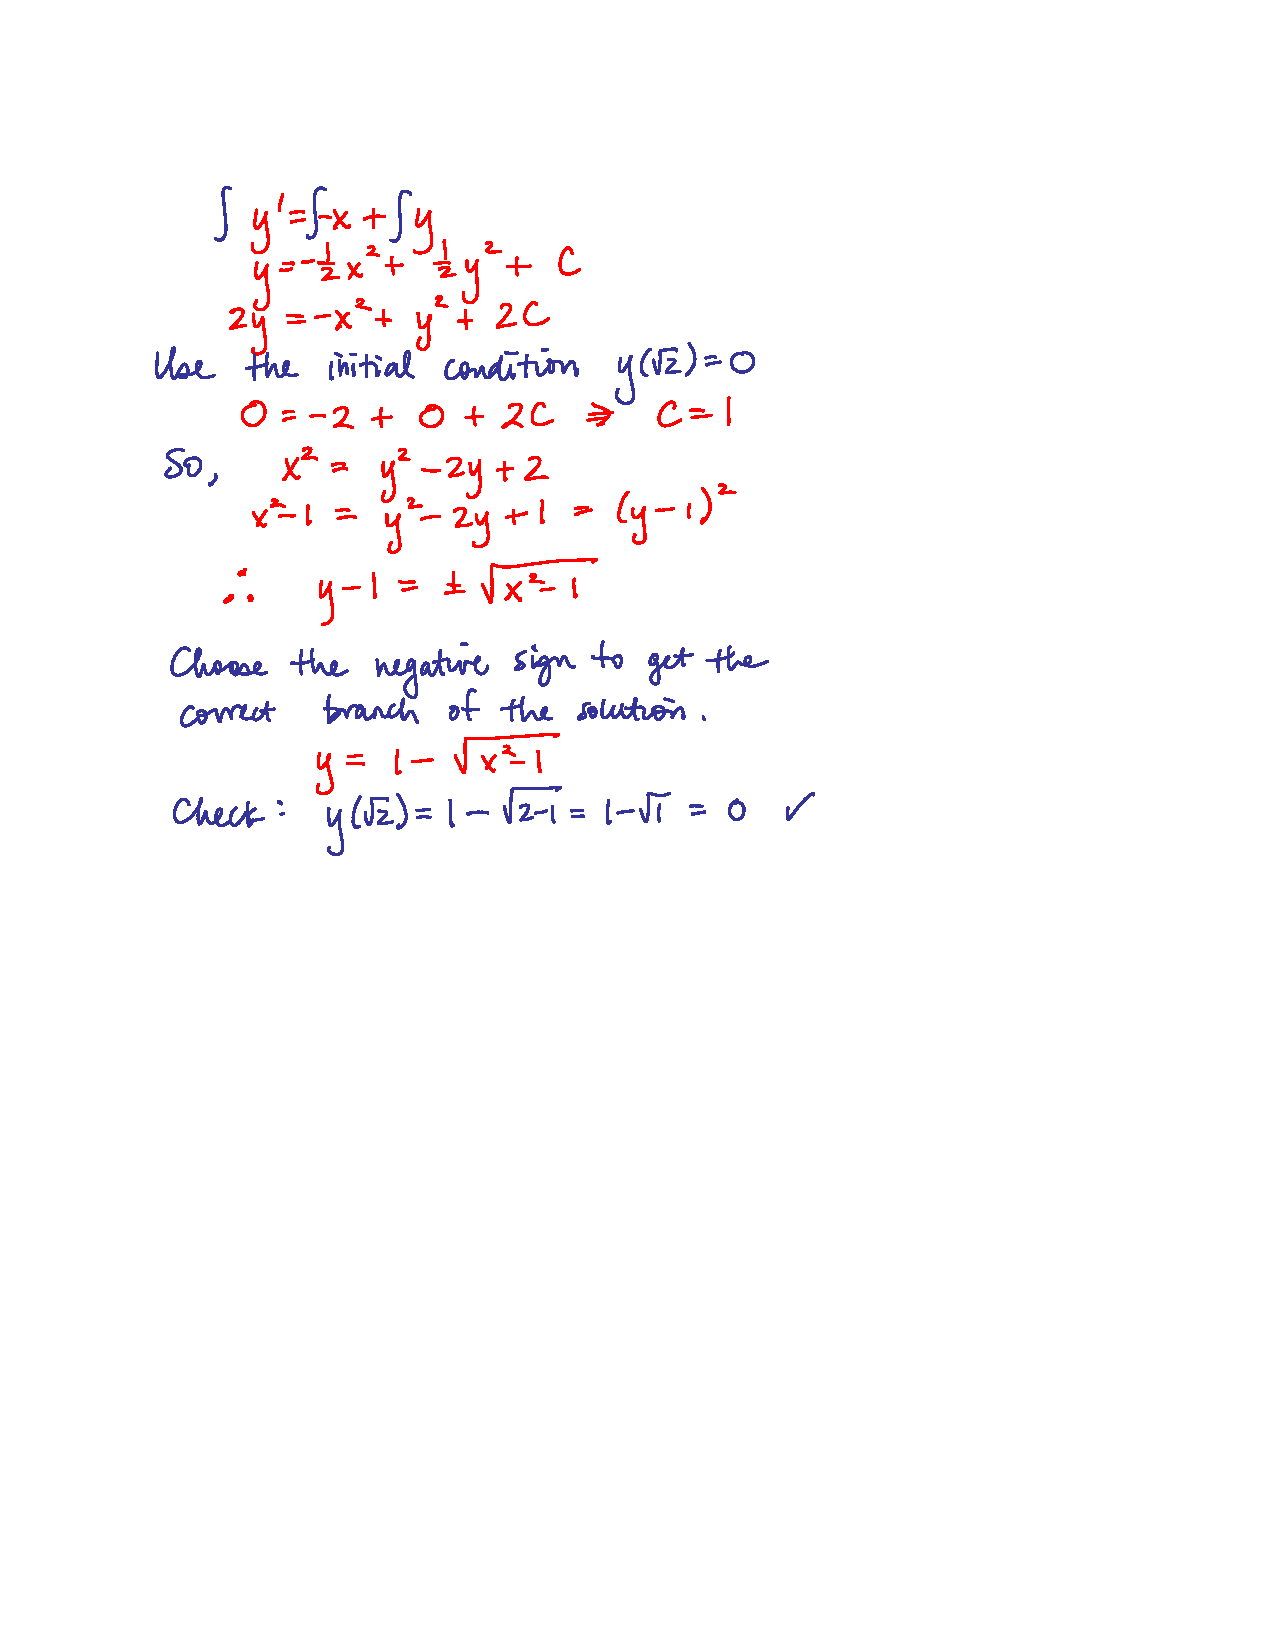
\includegraphics[width=3in,keepaspectratio=true]{img/apr_15_1.pdf}}}
    \end{center}
\end{problem}

%p1%
\begin{solution}
    \vfill
\end{solution}
\newpage

%p2%
\begin{problem}[2]
    At midnight, it is $20^\circ$F outside and $70^\circ$F inside
    when your furnace breaks. Two hours later, the temperature inside
    has fallen to $60^\circ$F. 

    \begin{center}
        \framebox{\parbox[c]{6in}{\textbf{Newton's Law of Cooling:} The rate of change of the
                temperature of something is proportional to the temperature difference
                between that thing and its surroundings.
        }}
    \end{center}

    \begin{enumerate}
        \item Assuming that the temperature inside the house obeys Newton's
            Law of Cooling and that it stays $20^\circ$F outside, determine the
            temperature inside the house as a function of time. When will it
            reach $40^\circ$F inside the house?
        \item Clearly the temperature outside won't stay constant.  Suppose that we model the temperature as a sinusoidal function with a minimum value of $20^\circ$F at midnight and a maximum value of $40^\circ$F at noon.  Determine the temperature inside the house and time the house will reach $40^\circ$F under these assumptions.  (Note: To solve for the time to reach $40^\circ$F in this situation, you will need to solve a nonlinear equation.  You can use a graph to estimate the solution to this equation, or you can use a computer to approximate the solution for you. Feel free to use \texttt{fsolve} in Matlab or \texttt{FindRoot} in Mathematica.)
        \item What other assumptions could be relaxed to produce a more accurate prediction?  You could also earn some extra credit here if you rework the problem again using your ideas.
    \end{enumerate}
\end{problem}

\begin{solution}
    \vfill
\end{solution}
\newpage

%p3%
\begin{problem}[3]
    Use the Wronskian to determine whether the following functions $y_1$ and $y_2$ are linearly independent or linearly dependent on the interval $t \in (0,1)$.
    \begin{enumerate}
        \item $y_1(t) = e^{5t}, \ y_2(t)=e^{-3t}$
        \item $y_1(t) = t^2, \ y_2(t) = t^4 $
        \item $y_1(t) = \cos t \sin t, \ y_2(t) = \sin 2t$
        \item $y_1(t) = e^{\alpha t} \cos \beta t, \ y_2(t) = e^{\alpha t} \sin \beta t \quad (\alpha,\beta \text{ constants}, \beta \neq 0)$
    \end{enumerate}
\end{problem}

\begin{solution}
    \vfill
\end{solution}
\newpage

%p4%
\begin{problem}[4]
    Consider the equation 
    \begin{equation*}
        y'' + p(t) y' + q(t) y = 0, \qquad t \in I,
    \end{equation*}
    where $p(t)$ and $q(t)$ are continuous on $I$. Let $y_1$ and $y_2$ be
    solutions to this equation.  
    \begin{enumerate}
        \item Prove that if $y_1$ and $y_2$ are zero at the same point in $I$,
            then they cannot be a  \textit{fundamental set} on $I$.
        \item Prove that if $y_1$ and $y_2$ have maxima or minima at the same
            point in $I$, then they cannot be a \textit{fundamental set} on $I$.
    \end{enumerate}
\end{problem}

\begin{solution}
    \vfill
\end{solution}
\newpage

%p5%
\begin{problem}[5]
    Examine Student R's work on the following problem.  What did the student do correctly?  What mistake(s) did the student make?  (There are at least three.) What is a more correct response to the problem, and what would you say to help the student understand how to correctly complete the problem?

    \begin{center}
        \framebox{\parbox[c]{5.5in}{Determine the general solution to the DE $xy'+2y=\sqrt{x}$.

        \centering\includegraphics[width=3in,keepaspectratio=true]{img/apr_15_5.pdf}}}
    \end{center}
\end{problem}

\begin{solution}
    \vfill
\end{solution}
\end{document}
